\documentclass[12pt,letterpaper]{article}
\usepackage[latin1]{inputenc}
\usepackage[spanish]{babel}
\usepackage{graphicx}
\usepackage[left=2cm,right=2cm,top=2cm,bottom=2cm]{geometry}
\usepackage{graphicx} % figuras
\usepackage{subfigure} % subfiguras
\usepackage{float} % para usar [H]
\usepackage{amsmath}
\usepackage{txfonts}
\usepackage{stackrel} 
\usepackage[latin1]{inputenc}
\usepackage{multirow}
\usepackage{enumerate} % enumerados
\renewcommand{\labelitemi}{$-$}
\renewcommand{\labelitemii}{$\cdot$}
\author{Nelia Escalante}
\title{Caratula}
\begin{document}

\title{Caratula}

\begin{titlepage}
\begin{center}
\large{UNIVERSIDAD PRIVADA DE TACNA}\\
\vspace*{-0.025in}
\begin{figure}[htb]
\begin{center}

\includegraphics[width=11cm]{./IMG/logo}
\end{center}
\end{figure}
\Large INGENIERIA DE SISTEMAS  \\

\vspace*{0.5in}
\begin{large}
\textbf{TITULO:} \\
\end{large}

\vspace*{0.1in}
\begin{Large}
\textbf{Modelado de Datos en Power BI} \\
\end{Large}

\vspace*{0.3in}
\begin{Large}
\textbf{CURSO:} \\
\end{Large}

\vspace*{0.1in}
\begin{large}
INTELIGENCIA DE NEGOCIOS\\
\end{large}

\vspace*{0.3in}
\begin{Large}
\textbf{DOCENTE:} \\
\end{Large}

\vspace*{0.1in}
\begin{large}
 Ing. Patrick Cuadros Quiroga\\
\end{large}

\vspace*{0.2in}
\vspace*{0.1in}
\begin{large}
\textbf{ESTUDIANTE:} \\
\vspace{\baselineskip}
\begin{flushleft}

Escalante Maron, Nelia 		\hfill	(2014049551) \\

\end{flushleft}
\end{large}
\end{center}

\end{titlepage}

\newpage

	\begin{center}
		\Large Modelado de Datos en Power BI
	\end{center}
	\vspace{\baselineskip}
	\vspace{\baselineskip}
	\textbf{\Large 1. RESULTADOS DEL DESARROLLO:}
	\\\\
Al desarrollar los pasos anteriores de la practica, veremos y mostraremos los resultados siguientes, indicando los pasos que se desarrollaron. \\\\


1. Iniciar Power BI Desktop.\\\\ 
2. En la Ventana de Power BI Desktop, click en Obtener Datos (Get Data).\\\\ 
3. En el cuadro de dialogo Obtener Datos (Get Data), asegurarse que Excel esta seleccionado y hacer click en Conectar (Connect).\\\\ 
4. En el cuadro de dialogo Abrir (Open), buscar el archivo Adventure Works Sales Data.xlsx, y luego hacer click en Abrir (Open).\\\\ 
5. En el cuadro de dialogo Explorador (Navigator), seleccionar las hojas DimCurrency, DimCustomer, DimDate, DimProduct, DimPromotion, DimSalesTerritory, y FactInternetSales.\\\\ 
\begin{center}
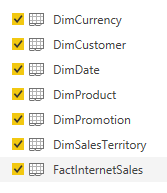
\includegraphics[width=9cm]{IMG/2.png} 
\end{center}
6. Hacer click en Cargar (Load).\\\\ 
7. En el panel de vistas a mano derecho, hacer click en Relaciones (Relationships).\\\\ 
\begin{center}
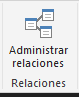
\includegraphics[width=5cm]{IMG/3.png} 
\end{center}
8. En el menu principal, hacer click en Administrar relaciones (Manage Relationships).\\\\ 
9. En el cuadro de Administrar relaciones (Manage Relationships), hacer click en Nueva (New).\\\\ 
10. En el cuadro de Administrar relaciones (Manage Relationships), en la lista de tablas superior, hacer click en FactInternetSales. Cuando la vista previa de la table aparezca hacer click en la columna OrderDateKey.\\\\ 
11. En la lista de table inferior, hacer click en DimDate. Cuando la vista previa de la table aparezca hacer click en la columna DateKey.\\\\ 
12. Revisar que la cardinalidad (Cardinality) esta seleccionada para Muchos a Uno (Many to One), que la Direccion del filtro cruzado (Cross filter direction) es Sencilla (Single), y que la opcion Hacer esta relacion activa (Make this relationship active) se encuentra seleccionada, luego hacer click en Aceptar (OK).\\\\ 
\begin{center}
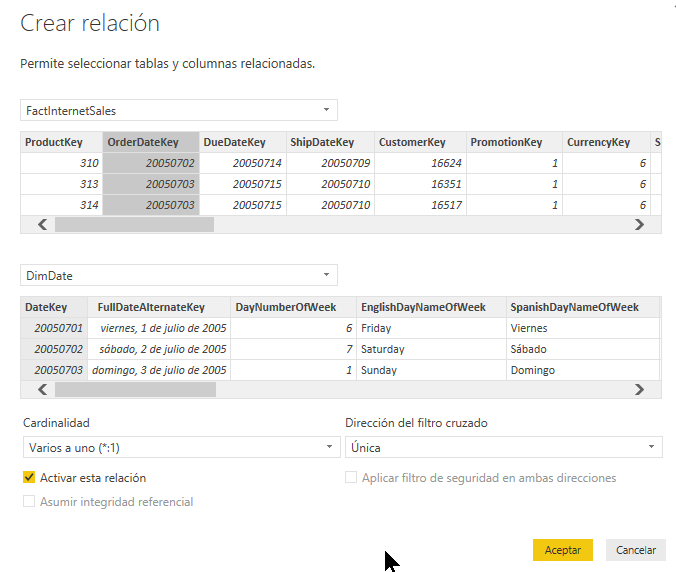
\includegraphics[width=13cm]{IMG/4.png} 
\end{center}
13. En el cuadro de Administrar relaciones (Manage Relationships), hacer click en Cerrar (Close).\\\\ 
14. En el diagrama, en la tabla FactInternetSales, hacer click en la columna DueDateKey. Arrastrar la columna
DueDateKey a la columna DateKey de la tabla DimDate.\\\\ 
15. En el diagrama, en la tabla FactInternetSales, hacer click en la columna ShipDateKey. Arrastrar la
columna ShipDateKey a la columna DateKey de la tabla DimDate.\\\\ 
16. En el menu principal, hacer click en Administrar relaciones (Manage Relationships).\\\\ 
17. En el cuadro de Administrar relaciones (Manage Relationships), hacer doble click en la relacion
FactInternetSales (CurrencyKey).\\\\ 
18. En la lista de Direccion de Filtro Cruzado (Cross filter direction), hacer click en Sencilla (Single), luego
hacer click en Aceptar (OK).\\\\ 
19. En el cuadro de Administrar relaciones (Manage Relationships), hacer doble click en la relacion
FactInternetSales (ProductKey).\\\\ 
20. En la lista de Direccion de Filtro Cruzado (Cross filter direction), hacer click en Sencilla (Single), luego
hacer click en Aceptar (OK).\\\\ 
21. En el cuadro de Administrar relaciones (Manage Relationships), hacer doble click en la relacion
FactInternetSales (PromotionKey).\\\\ 
22. En la lista de Direccion de Filtro Cruzado (Cross filter direction), hacer click en Sencilla (Single), luego
hacer click en Aceptar (OK).\\\\ 
23. En el cuadro de Administrar relaciones (Manage Relationships), hacer doble click en la relacion
FactInternetSales (SalesTerritoryKey).\\\\ 
24. En la lista de Direccion de Filtro Cruzado (Cross filter direction), hacer click en Sencilla (Single), luego
hacer click en Aceptar (OK).\\\\ 
25. En el cuadro de Administrar relaciones (Manage Relationships), hacer click en Cerrar (Close).\\\\ 
26. Hacer click en la linea de relacion entre FactInternetSales and DimCustomer y presionar Borrar (Delete).\\\\ 
27. En el cuadro de dialogo Eliminar relacion (Delete Relationship), hacer click en Borrar (Delete).\\\\ 
28. En el menu principal, hacer click en Administrar relaciones (Manage Relationships).\\\\ 
29. En el cuadro de Administrar relaciones (Manage Relationships), hacer click en Nueva (New).\\\\ 
30. En la lista de tablas superior, hacer click en FactInternetSales. Luego hacer click en la columna
CustomerKey en la vista de datos previa.\\\\ 
31. En la lista de tablas superior, hacer click en DimCustomer, y hacer click CustomerKey en la vista de datos
previa.\\\\ 
32. En la lista de Cardinalidad (Cardinality), hacer click en Muchos a Uno (Many to One), y luego hacer
click en Aceptar (OK).\\\\ 
33. En el cuadro de Administrar relaciones (Manage Relationships), hacer click en Cerrar (Close).\\\\ 
34. Hacer click en Guardar (Save), y cuargar el archive como Ventas Adventure Works.pbix.\\\\ 

Parte 2: Relaciones Manuales\\\\
1. En la Ventana de Power BI Desktop, click en Obtener Datos (Get Data) y luego en Excel.\\\\
2. Abrir el archivo Adventure Works Product Categories.xlsx.\\\\
3. En el cuadro de dialogo Explorador (Navigator), seleccionar las hojas DimProductCategory, and
DimProductSubcategory, y luego hacer click en Cargar (Load).\\\\
\begin{center}
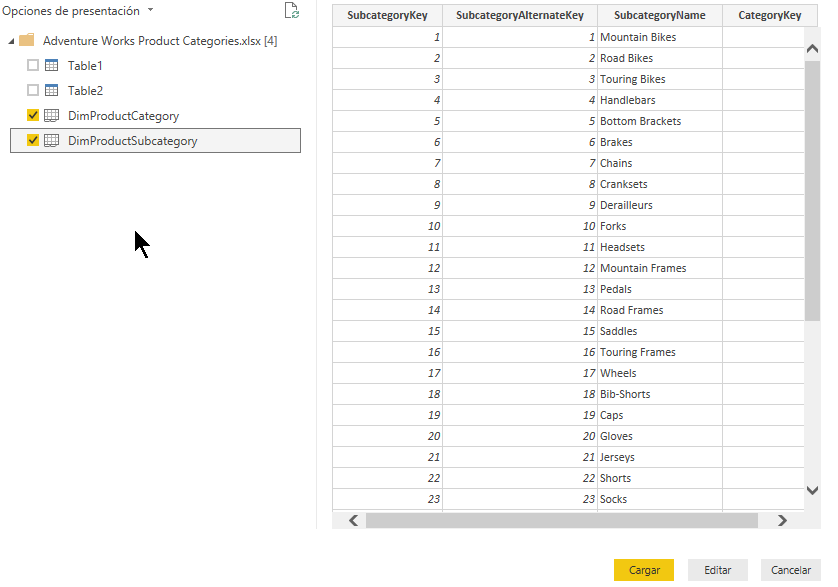
\includegraphics[width=15cm]{IMG/5.png} 
\end{center}
4. En el panel de Relaciones, revisar la relacion que Power BI ha creado entre las dos tablas.\\\\
\begin{center}
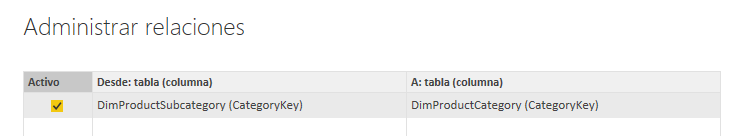
\includegraphics[width=15cm]{IMG/6.png} 
\end{center}
5. Hacer click en la linea de la relacion entre DimProductCategory, y DimProductSubcategory, y seleccionar
Eliminar (Delete).\\\\
\begin{center}
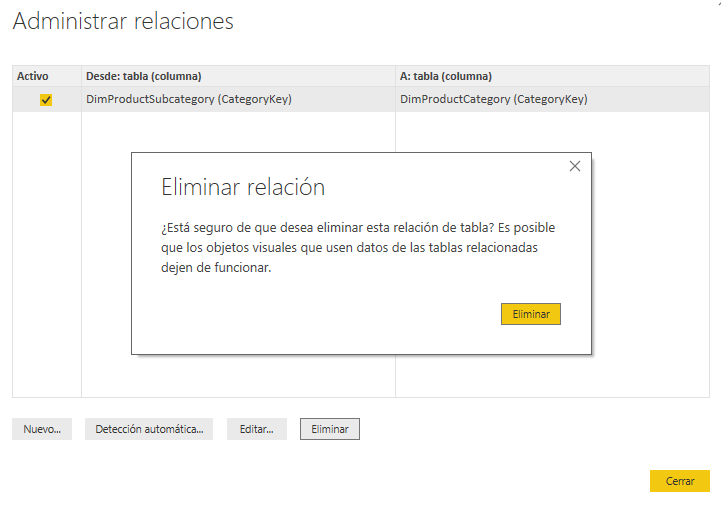
\includegraphics[width=15cm]{IMG/7.png} 
\end{center}
6. En el cuadro de dialogo Eliminar relacion (Delete Relationship), hacer click en Borrar (Delete).\\\\
\begin{center}
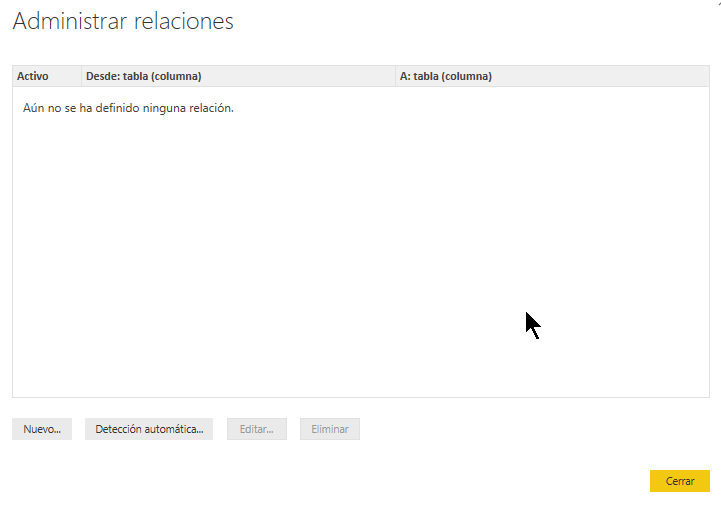
\includegraphics[width=15cm]{IMG/8.png} 
\end{center}
7. Arrastrar la columna CategoryKey en la tabla DimProductSubcategory a la columna Category en la tabla
DimProductCategory, para crear una relacion Muchos a uno (Many to One ), y una direccion de filtro
cruzado (Cross filterdirection) en ambos.\\\\
8. En la tabla DimProduct, arrastrar la columna ProductSubcategoryKey a la columna SubcategoryKey en la
tabla DimProductSubcategory, para crear una relacion de Muchos a Uno (Many to One ), y una direccion de filtro cruzado (Cross filter direction) en ambos.\\\\
\begin{center}
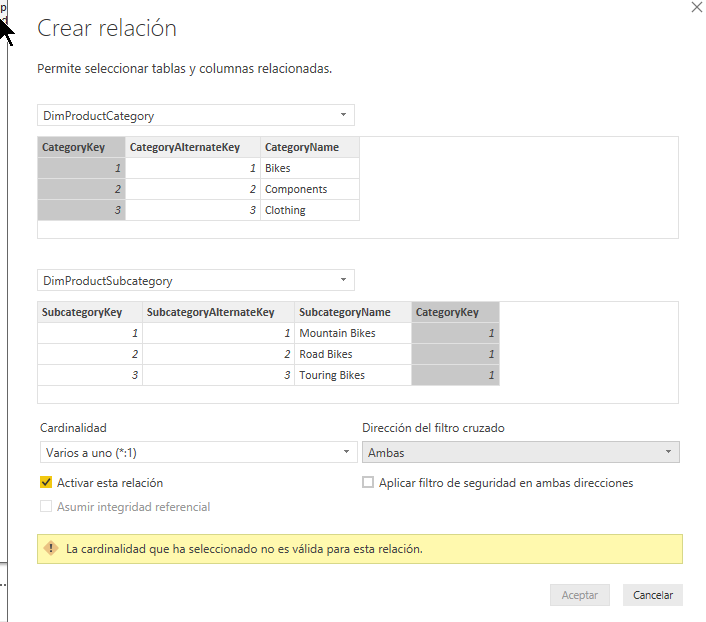
\includegraphics[width=15cm]{IMG/9.png} 
\end{center}
9. Hacer click en Guardar\\\\


\end{document}